\chapter{Electrical transport experimental design \label{chap:elec}}
\textit{In situ}, four probe, gate dependent electrical transport measurements can be used to measure the phonon induced electrical band gap discussed in Chapter \ref{chap:kek}.
The fingerprint of the phonon induced band gap is transport phenomena which are corrolated with the creation of the Kekul\'e phonon.
In this Appendix gated electrical transport is considered, the expected changes in the electrical transport of gapped graphene is discussed, and finally the measurement of gated electrical transport is described in detail.

\section{Gate dependent transport}
The resistance, $R$, of a graphene device is related to the two dimensional resistivity, $\rho$, and the two dimensional conductivity, $\sigma$, through
\begin{equation*}
	\rho=\frac{1}{\sigma}=R \frac{w}{L} \ ,
\end{equation*}
where $w$ is the width and $L$ is the length of the measured graphene strip.
To differentiate resistance and resistivity, the units of resistivity are written as $\Omega/\square$.
Gate dependent resistance measurements provide information about a graphene device.

Graphene's two dimensional nature makes it simple to continuously modify the Fermi energy using a back gate.
Rather than varying the concentration of a dopant as must be done for most three dimensional systems, graphene's Fermi energy can be capacitively tuned with a back gate, as shown schematically in Figure \ref{fig:kek:FET}.
Together, the silicon back gate and the graphene form a parallel plate capacitor with a plate separation of 285 nm and the dielectric constant of thermal dioxide.
Changing the back gate voltage, $V_{BG}$, adds or removes a charge of $n=CV_{BG}/e$ to the graphene where $C$ is the capacitance and $e$ is the charge of the electron.
When $V_{BG}$ is set such that the Fermi energy sits at the charge neutrality point there are the fewest number of charge carriers and thus the highest resistance.
This situation doesn't always correspond to $V_{BG}=0$; every device has a finite number of dopants which shift the Dirac point from zero volts.
Tuning the back gate voltage away from the Dirac point adds additional charges and lowers the resistance.

\begin{figure}
	\begin{center}
	\newcommand{\FEThw}{4 cm}			% Width--1 cm=1 um
\newcommand{\FETsiot}{.3 cm}		% SiO2 thickness
\newcommand{\FETsit}{.7 cm}			% Si thickness
\newcommand{\FETaut}{0.06 cm}		% Au thickness
\newcommand{\FETauw}{2 cm}			% Separation and width of the gold pad
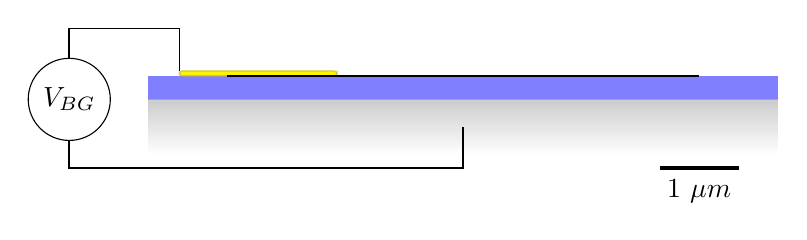
\begin{tikzpicture}[scale=1,
	sio2/.style={fill=blue!50!white,draw=none},
	si/.style={top color=black!20!white, bottom color=white},
	siedge/.style={draw=black!35!white},
	au/.style={fill=yellow,draw=black!20!yellow,rounded corners=1 pt},
	wire/.style={semithick}]
	
	%The SiO2
	\filldraw[sio2] (-\FEThw,0) rectangle (\FEThw,\FETsiot);

	%The Si
	\shade[si] (-\FEThw,-\FETsit) rectangle (\FEThw,0);
	\draw[siedge] (-\FEThw,0) -- (\FEThw,0);

	%The Gold contacts
	\filldraw[au] (-\FEThw*.9,\FETsiot) rectangle +(\FETauw,\FETaut);
	
	%The Graphene on the top
	\draw[semithick] (-3*\FEThw/4,\FETsiot) -- (3*\FEThw/4,\FETsiot);

	%The wires connecting the gate etc.
	\node (VBG) at (-1.25*\FEThw,0) [circle,draw=black]{$V_{BG}$};
	\draw[wire]  (VBG.north) -- (-1.25*\FEThw,2.5*\FETsiot+2.5*\FETaut) -- (-\FEThw*.9,2.5*\FETsiot+2.5*\FETaut) -- (-\FEThw*.	9,\FETsiot+\FETaut);
	\draw[wire]  (VBG.south) -- (-1.25*\FEThw,-1.25*\FETsit) -- (0,-1.25*\FETsit) -- (0,-.5*\FETsit);

	%Scale bar
	\draw[draw=black,ultra thick,xshift=.75*\FEThw, yshift=-\FETsit*1.25] (-.5 cm,0) -- node[anchor=north] {$1 \ \mu m$}(.5 cm, 0);

\end{tikzpicture}
	\end{center}
	\caption[Side view of a back gated graphene device.]{\label{fig:kek:FET} 
	Side view of a back gated graphene device.
	The contacted graphene (black line) is on top of 285 nm of thermal oxide (blue) grown on heavily doped silicon (gray).
	A voltage difference of $V_{BG}$ is placed between the silicon and the graphene to drive charges into the graphene.
	}	
\end{figure}

Near the Dirac point in gapless graphene the conductivity is symmetric and nearly linear allowing a field effect mobility, $\frac{d \sigma}{d (n e)}$, to be defined.
Even though there are no charge carriers at the Dirac point there is always a residual conductivity, $\sigma_0$ \cite{DasSarma2011}.
Further from the Dirac point the conductivity is sub-linear and is best fit by
\begin{equation*}
	\frac{1}{\sigma}=\frac{1}{n e \sigma_C + \sigma_0} + \rho_S \ ,
\end{equation*}
where $\mu_C$ is the mobility due to long-range Coulomb scattering and $\rho_S$ is from short range scattering \cite{Dean2010,DasSarma2011,Remi2013T}.
Higher quality devices have higher mobilities and Dirac points closer to $V_{BG}=0$.

For gapless graphene, the Fermi energy can be determined from $V_{BG}$ by matching the integrated density of states (Equation \ref{eq:TB:DOS}) to $n$.
Some useful relationships for graphene on 285 nm of thermal oxide are
\begin{align*}
	n(cm^{-2})&\sim 7 \times 10^{10} V_{BG} (Volts) \\
	\mu(meV) &\sim 30 \sqrt{V_{BG} (Volts)} \\
	\mu(meV) &\sim 1 \times 10^{-7} \sqrt{n(cm^{-2})} \ ,
\end{align*}
where $\mu$ is the Fermi energy.

\section{Electrical transport fingerprints of the phonon induced band gap}
The opening of the band gap should have two fingerprints in electrical transport.
First, the resistance at the charge neutrality point should increase.
If the capability were available, measuring the temperature dependence of this resistance would give a direct measurement of the size of the band gap.
Second, because of the energy required to excite an electron across the band gap, the gate dependent conductivity should exhibit a low conductivity plateau centered on the charge neutrality point.
The width of this plateau in volts should correspond to the band gap in electron volts plus any many body effects.
The corrolation of these fingerprints with the excitation of the Kekul\'e phonon would be proof of the phonon induced band gap.

\section{Measurement of the gate dependent electrical transport}
When performing these measurements the goals are to achieve sufficient signal to noise while protecting the nanomaterial from damage.
In this Appendix the devices used to measure the transport, the precautions employed to protect the graphene, and the methods of shielding the electronics are described.
Because of its importance and because it is so easily forgotten, it should be immediately mentioned that a grounding strap should always be worn when measuring graphene's electrical properties.

A circuit diagram detailing the electronic devices is shown in Figure \ref{fig:elec:wires}.
A Standford Research SR850 digital lock-in is used to measure the low frequency AC resistance of the graphene device in the four probe, Kelvin sensing geometry.
The variable back gate voltage is supplied by a Keithley 2400 source meter (K2400).
The breakout box is a custom built passive electronics box that serves several functions.
It has two double pull switches, $S_1$ and $S_2$, used to ground and protect the sample.
It also holds the current limiting $10 M \Omega$ resistor.
Finally, it breaks the six core, shielded, sample connection wire into six individual BNC terminals.
Using short BNC jumpers these terminals are connected to the second row of BNC terminals allowing for a flexible connection between the sample and the source voltage, $S$, the drain voltage, $D$, the voltage measurement probes, $V_1$ and $V_2$, and the back gate voltage, $V_{BG}$.
All grounds in the system are connected to the SR850 ground.
These electronic devices will be described in some detail below.

\begin{figure}
	\begin{center}
	{
\begin{tikzpicture}[on grid,
	boxstyle/.style={rounded corners=2.5pt,thick},
	grndstyle/.style={color=green!70!black}
	]
	% The SR850
	\begin{scope}
		\node[circ]			(Sin)		[label={[align=center]right:Sine\\Out}] 	at (0,0)	{};
		\node[circ]			(Ain)		[label=right:$A$]		at (2,0)	{};
		\node[circ]			(Bin)		[label=right:$B$]		at (3,0)	{};
		\draw[boxstyle] (-.5,-.5) rectangle (4,1) node[anchor=north east] {SR850};
	\end{scope}

	% The Keithley 2400
	\begin{scope}[xshift=-5cm]
		\node[circ]			(Hi)		[label=right:$Hi$] 	at (0,0)	{};
		\node[circ]			(Lo)		[label=right:$Lo$] 	at (1,0)	{};
		\draw[boxstyle] (-.5,-.5) rectangle (2,1) node[anchor=north east] {K2400};
	\end{scope}

	% The breakout box
	\begin{scope}[yshift=-5 cm]
		% The outputs
		\node[ocirc]			(Sout)		[below=5cm of Sin.center, anchor=center,label=right:$S$] 		{};
		\node[ocirc]			(Dout)		[right=1cm of Sout.center,anchor=center,label=right:$D$] 		{};
		\node[ocirc]			(VBGout)	[left= 1cm of Sout.center,anchor=center,label=right:$V_{BG}$] 	{};
		\node[ocirc]			(V1out)		[below=5cm of Ain.center, anchor=center,label=right:$V_1$]		{};
		\node[ocirc]			(V2out)		[below=5cm of Bin.center, anchor=center,label=right:$V_2$]		{};

		% The switches
		% S1
		\node[spdt,rotate=90]	(dpdt1)		[above=1cm of Sout.center  ,anchor=in] {};
		\node[spdt,rotate=90]	(dpdt2)		[above=1cm of VBGout.center,anchor=in] {};
		\draw[grndstyle] (dpdt2.out 2)	to[R=$10 \Omega$,bipoles/length=.5cm] +(0,.5cm) node[sground,rotate=180] (gnd1) {};
		\draw[grndstyle] (dpdt1.out 2) -- (dpdt2.out 2);
		\draw[thick,dashed] ($(dpdt2.center) +(-.5cm,0)$) node[anchor=north east]{$S_1$} -- ($(dpdt1.center) +(.5cm,0)$);
		% S2
		\draw ($(Bin.center)+(0,-3cm)$) to[short,*-] ++(+.3cm,0) to[cspst,-o] ++ (0,.5cm) node[sground,rotate=180,grndstyle] (gnd2) {}; 
		\draw ($(Ain.center)+(0,-3cm)$) to[short,*-] ++(+.3cm,0) to[cspst,-o] ++ (0,.5cm); 
		\draw[grndstyle] ($(Ain.center)+(0,-3cm)+(+.3cm,0)+(0,.5cm)$) -- (gnd2.center);
		\draw[thick,dashed] ($(Ain.center)+(-.25cm,-2.75cm)$) node[anchor=north east]{$S_2$} -- ($(Bin.center)+(.5cm,-2.75cm)$);

		% Limiting resistor
		\draw (Sin.center) to[R=$11 M\Omega$]	+(0,-2.5cm) -| (dpdt1.out 1);

		% Ground for drain
		\draw[grndstyle] (Dout.center) -- +(0,.25cm) node[sground,rotate=180] {};

		% The connections
		\draw (dpdt1.in)	--		(Sout.center);
		\draw (dpdt2.in)	--		(VBGout.center);
		\draw (Hi.center)	|-		(dpdt2.out 1);
		\draw[grndstyle] (Lo.center)	|- (gnd1.center);
		\draw (Ain.center) -- (V1out.center);
		\draw (Bin.center) -- (V2out.center);

		% An array of open circles across the bottom for the break out
		\foreach \ip/\ilab in {-2.5cm/G1,-1.5cm/G2,-.5cm/G3,.5cm/G4,1.5cm/G5,2.5cm/G6} {
			\node[ocirc] (\ilab) [below right=1 cm and \ip of Dout.center, anchor=center, label=right:\ilab]	{};
		}

		% Wiring these circles into a thick wire
		\foreach \ilab in {G1,G2,G3,G4,G5,G6}{
			\draw (\ilab.center) |- ($(Dout.center)-(0,1.5cm)$);
		}

		% Wire connecting to the vacuum chamber---didn't do a great job with these
		\draw[ultra thick] ($(Dout.center)-(0,1.5cm)$) -- ($(Dout.center)-(0,4.6cm)$);
		\draw[grndstyle] ($(Dout.center)-(+0.1cm,2.0cm)$) -- ($(Dout.center)-(+0.1cm,4.6cm)$);
		\draw[grndstyle] ($(Dout.center)-(-0.1cm,2.0cm)$) -- ($(Dout.center)-(-0.1cm,4.6cm)$);

		% Bounding rectangle
		\draw[boxstyle] ($(G1.center)-(1cm,1cm)$) rectangle ($(G6.center|- Bin)+(1.5cm,-.6cm)$) 
			node[anchor=north east,align=center]	{Break \\ Out\\Box};
	\end{scope}

	% Inside the Vacuum Chamber
	\begin{scope}[xshift=1cm,yshift=-10.5cm]
		\draw[boxstyle] (-2.5cm,-2.5cm) rectangle (2.5cm,2.5cm) node[anchor=north east,align=center] {Test\\Cube};
		\draw (-.9cm,-.9cm) rectangle (.9cm,.9cm);

		% The pins to the sample
		\foreach \x/\y/\lab/\dir in {.4/.75/G1/above,-.4/.75/G2/above,-.75/.4/G3/left,-.75/-.4/G4/left,-.4/-.75/G5/below,.4/-.75/G6/below,.75/-.4//right,.75/.4//right}{
			\node[ocirc] at (\x,\y)  [label=\dir:\lab] {};
		}
	\end{scope}

\end{tikzpicture}
}
	\end{center}
	\caption[Circuit diagram for graphene electrical transport measurements]{\label{fig:elec:wires}
		Circuit diagram of the electronics for measuring the phonon induced band gap in graphene.
		The diagram details the internal circuitry of the break out box which interfaces the Standford Research SR850 digital lock-in and the Keithley 2400 source meter with the graphene sample mounted in the test cube.
		The open $V_{BG}$, $S$, $D$, $V_1$, and $V_2$ contacts are bridged to the appropriate $G1-G6$ contacts using BNC jumpers.
		Switches $S_1$ and $S_2$ are used to ground the sample contacts.
		The grounds, colored in green, are all referenced to the SR850 ground.
		Although not shown in the diagram, the core of all BNC cables are grounded on one side.
	}
\end{figure}

The low frequency lock-in technique improves on the signal to noise of a DC measurement.
However, out of necessity the AC technique is slightly different than the traditional four probe DC resistance measurement.
This is because there is no such thing as a constant current AC sources which can be used to pump a contact resistant independent current from source to drain.
Instead, the effect of the contact resistance is minimized using a large resister, $R_L=11.130 M\Omega$, placed between the SR850 oscillator out and the source terminal as shown in Figure \ref{fig:elec:min}.
As long as the contact resistance is much less than $R_L$, the contact resistance can be ignored and the system can be treated as a voltage divider with the graphene resistance given by
\begin{equation*}
	R_g=R_{L} \frac{V_1-V_2}{V_{AC}-(V_1-V_2)} \pm R_{L} \left( \frac{V_{AC}}{(V_{AC}-(V_1-V_2))^2} \right) \delta (V_1-V_2) \ ,
\end{equation*}
where $V_{AC}=1$ is the root mean squared AC voltage amplitude used in experiments and the term after the $\pm$ is the standard error which is proportional to the uncertainty in the measured voltage, $\delta (V_1-V_2)$, determined by the standard deviation of $>10$ sequentially measured values.
The accuracy of this formula is limited if the resistance approaches the $10 M\Omega$ input impedance of the lock-in.
When $R_g<<R_L$ the useful approximation
\begin{equation*}
	R_g \approx (V_1-V_2) * 10^4 \frac{\Omega}{mV} \ ,
\end{equation*} 
holds.
The added resistor is useful for other reasons.
It limits the current through the graphene to a safe value of less than $100 nA$.
Additionally, the large value of $R_L$ ensures that the $50 \Omega$ output impedance of the lock-in is unimportant.
The resistor $R_L$ allows us to use lock-in techniques to increase our signal to noise.

To reduce noise in our measurements, we use the lock-in's internal oscillator as both the AC voltage source, $V_{AC}$, and as the reference to which the voltage measurements are mixed.
To limit AC cross talk between lines the source is set to oscillate at the relatively low value of $f=17 \ Hz$.
To best limit any 1/f noise the rule of thumb is to set the time constant of the low pass filter to $\tau=5 \frac{1}{f} \approx 300 ms$.
However, we use $\tau=100 ms$ because it triples the measurement speed but does not substantially increase the noise.
At each back gate voltage we takes 2 seconds worth of data sampled at $f_S=8Hz<=1/\tau$ and record the average and standard deviation of these 16 data points.
Between back gate voltages we wait for the low pass filter to respond by waiting for $10 \tau$.
The back gate capacitor is much faster than the low pass filter, fully charging in micro seconds.
Noise is further reduced by measuring with the $60 Hz$ and $120 Hz$ line filters removed and the synchronous filter turned off.
We use the 24 dB/octave low pass filter with a sufficiently large 36 dB dynamic reserve.
The voltage is measured between the A and B lock-in terminals with their shells grounded.
Using these techniques we achieve a sufficient signal to noise of 2000 to 1 for a resistance of $1 k\Omega$.

\begin{figure}
	\begin{center}
	{
\newcommand{\gw}{.5cm}
\newcommand{\gh}{3.75cm}
\newcommand{\cw}{.4cm}
\newcommand{\enl}{1.5pt}
\begin{tikzpicture}
	% The graphene sheat with contacts
	% the sheat itself
	\draw[decorate,decoration={random steps,segment length=3pt, amplitude=1 pt}] [draw=blue!80!black,fill=blue!20!white]
		(-\gw/2,-\gh/2) rectangle (\gw/2,\gh/2);
	% Contacts
	\foreach \y/\rot/\rott in {-1.5cm/180/-90,-.5cm/0/90,.5cm/0/90,1.5cm/180/-90}{
		\shade[top color=yellow!60!black,shading angle=\rott,rotate=\rot,yshift=\y] 
			($(\gw/2*5,-\cw/2-\enl)$) rectangle ($(-1*\gw/2*1.5-\enl,\cw/2+\enl)$);
		\shade[top color=yellow!80!black,shading angle=\rott,rotate=\rot,yshift=\y] 
			($(\gw/2*5,-\cw/2)$) rectangle ($(-1*\gw/2*1.5,\cw/2)$);
	}

	% The electronics
	% Voltage probes
	\draw (\gw/2*3.5,+.5) to[short,-o] +(1.5cm,0) node[anchor=west]{$V_1$};
	\draw (\gw/2*3.5,-.5) to[short,-o] +(1.5cm,0) node[anchor=west]{$V_2$};

	% The emf connected to the resitor
	% \node[sinusoidal voltage source] (emf) at (0,0) {};
	\draw (-1*\gw/2*3.5,-1.5) -- ++ (-3cm,0) to[sV,l=$1V$] ++ (0,3cm) to[R=$R_L$] (-1*\gw/2*3.5,1.5);
\end{tikzpicture}
}
	\end{center}
	\caption[Simplified circuit diagram of four probe AC transport measurements]{\label{fig:elec:min}
		Simplified circuit diagram of the four probe AC transport measurement.
	}
\end{figure}

The K2400 source meter is used as an ambipolar voltage source to control the back gate voltage.
During measurement the back gate voltage is set by the Hi terminal.
The outputted voltage is referenced to the floating Lo terminal that is in turn tied to ground in the breakout box.
To limit electro magnetic interference (EMI) the Hi and Lo terminals are connected to the breakout box via separate BNC cables that have shields grounded on the breakout box side.
Instrument noise is minimized by auto ranging the voltage.
This keeps the voltage range as low as possible for each step in the back gate sweep.
To protect the sample the current compliance is kept low and the software warns the user if it is reached.
A value of $10 \ \mu A$ is low enough to protect the sample but high enough that the current needed to charge the capacitor does not cause a warning.
The current compliance being reached is an indicator of a leaky back gate.
Finally to avoid SiO$_2$ breakdown the voltage in volts should be kept below the oxide thickness in nanometers.
Applying these settings allows the K2400 to provide a safe and stable back gate voltage.

To protect the sample there are two double pull switches on the break out box which ground the sample.
This is useful both when mounting the sample and for putting the system in a safe state during measurement downtime.
The first switch, $S_1$, is a shorting rotary switch (NKK switches model number HS16-5SN-ND) which toggles the back gate and source terminals between measurement and ground modes.
In measurement mode the terminals are connected to the measurement instruments while in ground mode the terminals are connected to ground through a $10 \Omega$ resistor.
To make the transition between measurement and ground modes smoother for the sample, a shorting switch is used so that the second throw is made before the first throw is broken.
For additional sample safety, the K2400 voltage and the sine out voltage on the SR850 should be set to zero to minimize the voltage change when switching.
The small resistor between switch and ground limits the current flow between instrument and ground during the shorting action of the switch.
Without this the small difference between the instrument voltages and ground can cause a large current flow to ground.
The second switch, $S_2$, is a simple double pull single throw switch used to ground the $V_1$ and $V_2$ terminals.
The $A$ and $B$ terminals on the SR850 are high impedance ($10 M \Omega$) terminals and, as such, static charge could build up on these terminals and destroy the sample when it is connected.
Closing $S_2$ grounds the terminals, dissipating any static charge.
Used together these switches ground all of the pins on the sample.

Several precautions are made when mounting the sample.
As mentioned earlier, a grounding strap is always worn.
During sample transport the pins are embedded in a conducting foam to keep all contacts at the same voltage.
The sample is then removed from the foam for mounting in the presence of an ionizing fan.
Before the sample is mounted switches $S_1$ and $S_2$ are set so that all the contacts are grounded.
These precautions protect the sample from damage during mounting.

To limit EMI the shields on all of the BNCs are grounded on one side.
They are only grounded on one side so as to avoid ground loops.
In a perfect scenario the shield grounds would be isolated from the instrument ground.
However, we do not have this capability.
To further limit the EMI the length of the BNC cables is minimized.
In fact the break out box is connected directly to the SR850.
Finally, the metal break out box shields the passive electronics inside.

The measurement of the phonon induced band gap relies on the electronics detailed here.
The electronics setup should maximize signal to noise while protecting the fragile graphene.